Du point de vue architectural, à savoir de notre point de vue, le système que nous mettons en place au niveau de la couche applicative doit respecter plusieurs requis, notamment pour permettre à notre application d'être conforme aux normes juridiques du milieu médical. Les services prévus à cet effet apparaissent à la figure \ref{architecture}.
\\
\begin{figure}[h!]
	\hspace*{-2.5cm}
	\centering
	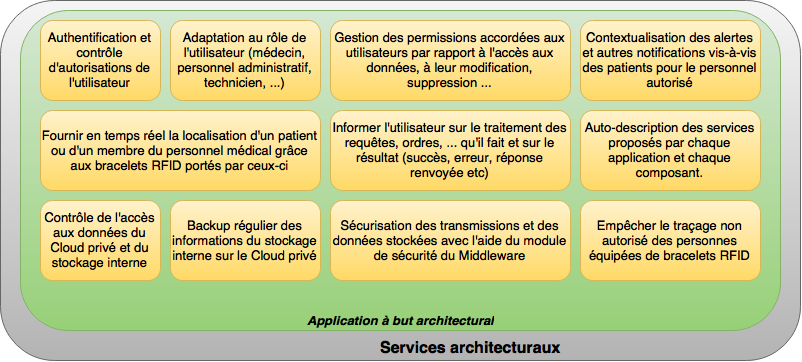
\includegraphics[width=1.4\textwidth]{architecture.png}
	\caption{Services de la Couche Applicative du côté de l'Architecture}
	\label{architecture}
\end{figure}

L'application proposée devra tout d'abord s’adapter, en terme de services proposés, à l’utilisateur, que ce soit le médecin, l'infirmier, la personne de la maintenance, le proche de la famille, ou l'hôpital. Ainsi, un système d’authentification est mis en place, et la personne devra s’identifier pour avoir accès aux services proposés. Chaque personne n’aura par conséquent pas les mêmes permissions, que ce soit en terme de visualisation des informations, mais aussi en terme de modifications de celles-ci. Ainsi, le médecin aura accès à l’historique des données et aux données courantes concernant le patient, et il pourra aussi apporter des modifications ; l’infirmier n’aura accès qu’aux données courantes ; la personne de la maintenance aura accès uniquement à l’historique des informations concernant les différents dispositifs utilisés ; l'hôpital aura accès à tout type d'informations et pourra les modifier afin de supprimer les informations périmées ou non utiles ; le proche de la famille pourra avoir accès aux informations non sensibles du patient afin d'avoir une connaissance de l'environnement du patient.

Au vue de ce qui a été dit précédemment, il faudra de l'interopérabilité à travers les différents services proposés, qui devront s'adapter à l'utilisateur.

Aussi, les informations et les permissions liées à celles-ci et fournies aux différents utilisateurs doivent dépendre de l’utilisateur. C'est pourquoi les permissions (modification, lecture, écriture) et les informations (log, informations liées aux patients) seront différentes selon l’utilisateur. L’application doit donc aussi restreindre les permissions concernant la modification ou la suppression des informations collectées, et cela en fonction de l'utilisateur.

Les informations liées au patient ne devront bien évidemment pas être anonymisées, mais au contraire contextualisées. En effet, si par exemple le médecin reçoit une alerte liée à un cas d'urgence, il faudra qu'il sache quel patient a généré cette alerte pour pouvoir le voir et gérer ce problème.

Notre système devra fournir la localisation des patients (grâce à leur puce RFID) qui est essentielle afin de savoir d'où provient une alerte ou une urgence (quel patient, et plus précisément quel capteur a généré telle information). La localisation du personnel médical (notamment grâce à la puce RFID des médecins) sera également fournie par le système, car elle est nécessaire pour attribuer une alerte ou une urgence à un personnel médical. Il faudra également gérer la localisation du personnel médical, car les déplacements générés par les médecins (et repérés par leur puce RFID) produisent des événements, et les services doivent s'adapter et prendre en considération ces événements (par exemple pour localiser le médecin le plus proche en cas d'urgence).

L’application devra fournir un feedback aux utilisateurs lorsque ceux-ci l'utilisent. Ce feedback servira à informer l’utilisateur que sa demande a été traitée, ou que l’indisponibilité du système n’a pas permis de traiter sa demande. Ce feedback devra être rapide dans le cas où les utilisateurs sont le personnel médical ou le personnel de maintenance (afin d'accélérer le traitement les alertes liées aux dispositifs ou au patient).

Les services proposés par l'application fourniront une auto-description, à savoir qu'ils donneront une description de ce qu'elles proposent (accès aux données, modification, historique, prise de rendez-vous, etc).

Comme indiqué précédemment dans le deuxième rapport, en plus d'un stockage interne, deux différents Cloud seront mis en place principalement pour le stockage des données. Le système intègrera tout d'abord un Cloud privé afin de stocker les informations sensibles et importantes, telles que les informations liées au patient et celles liées aux dispositifs et à leur état (les log). Ainsi, seuls les utilisateurs appartenant à l’hôpital (personnel médical, hôpital, personnel de maintenance) pourront y avoir accès. Le Cloud privé a la particularité par définition d'être isolé (car un seul et même serveur gère l’ensemble des données pour tous les utilisateurs), ce qui permet d'avoir une première protection et empêchera les attaques entre machines virtuelles (cross virtual machine attack). Étant donné que l'utilité du Cloud privé n'est liée qu'au stockage et à l'enregistrement (backup) d'informations, l'utilisateur n'aura tout simplement qu'à effectuer des requêtes pour avoir accès aux informations qu'il désire. C'est pourquoi l'utilisation du Cloud privé en tant que SaaS (Software as a Service) est suffisant, et l'application de gestion de données sera fournie par le fournisseur de ce Cloud.

Un Cloud public sera également utilisé au sein de notre système. Il stockera les informations non sensibles liées au patient et sera accessible par les proches du patient. Dans ce cas là, les données seront hébergées sur plusieurs serveurs eux-mêmes accessibles par un certain nombre d’utilisateurs, ce qui ne pose pas de problèmes ici car les informations stockées dans ce Cloud ne seront pas sensibles. Aussi, dans le Cloud public, en plus de l'application de gestion de données, nous fournirons une application d'authentification et de création de compte (pour permettre à chaque proche du patient d'avoir un compte), une application de rendez-vous (pour permettre aux proches du patient de prendre rendez-vous avec le médecin qui prend en charge le patient), et une application de messagerie instantanée (entre les proches du patient et le personnel médical). Comme nous fournirons dans ce Cloud l'application, nous aurons besoin d'un PaaS (Plateform as a Service).

Notre système devra automatiser le stockage des informations, depuis le stockage interne jusqu'au Cloud privé (avec un backup régulier, toutes les 6 heures par exemple) et public.

Afin de renforcer la sécurité et la confidentialité des informations (notamment celles liées au patient) dans les Cloud public et privé, il nous faudra crypter les informations stockées dans ces Cloud. L'accès aux informations liées au patient, au personnel médical et de maintenance, ainsi qu'aux ressources de l'hôpital (les dispositifs) devront être elles aussi sécurisées. C'est pourquoi toutes les communications vers les services proposés, vers les utilisateurs finaux, ainsi que toutes les communications provenant des services (et donc générées par les utilisateurs) devront être sécurisées. Comme dit précédemment, le Cloud privé servira aussi de backup (qui sera crypté), ce qui permettra une récupération sécurisée des informations en cas de problèmes. Afin de sécuriser et d'avoir un meilleur contrôle d'accès, et dans le cadre de l'authentification des utilisateurs, un identifiant unique sera fourni à chaque utilisateur. Notre système devra également rendre difficile l'espionnage de communication de messages à travers nos services, et devra empêcher le traçage des utilisateurs qui possèdent une puce RFID (médecin et patient) par des entités non autorisées, toujours pour améliorer la sécurité et la confidentialité. 

Enfin, notre système devra toujours permettre à un service d'être accessible par un utilisateur qui a le droit d'y accéder (pour assurer la disponibilité de notre application), et les informations qui circulent dans notre système devront être fiables, surtout en ce qui concerne les informations sensibles (qui peuvent potentiellement générées des alertes et des urgences liées au patient ou au dysfonctionnement des dispositifs).